\chapter{Discussion}

The results show that tracking a ground path using a camera fixed to a fixed wing UAV is a difficult task to solve, however, great improvements can be made by using optimization techniques.


\section{Piecewise Linear Vs. Curved Paths}

When optimizing the paths it was pretty clear that the MPC handles curved paths better than linear paths. The sharp corners of the linear paths caused troubles, and the MPC was not able to optimize corners sharper than about $45\degree$. Testing shows that the MPC might handle sharper corners if the stepsize is reduced.

For curved paths the turns can be a lot sharper. The MPC can handle $90\degree$ turns with a radius as low as $50$m. However, for longer $180\degree$ turns the results was not as good. The MPC handles the turns with a radius of $200$m, but below this the optimization fails.

When simulating the optimized paths in the simulator, the optimized paths for the piecewise linear paths turned out to be better than the curved paths. Both kinds shows great improvement from tracking the ground path itself.


\section{Oscillations (Working Title)}

The results in section \ref{sec:reducing_stepsize} show that when the stepsize is reduced, the oscillations in the states increase. This phenomenon is also present when using a stepsize of $0.2$s, but because of the longer time between every re-initiation the effect is not as visible as for $0.1$s.

A major contributor to generating these oscillations is the trajectory generator described in section \ref{subseq:generating_trajectory}, that assumes the UAV will maintain a fixed speed in order to calculate the distance the UAV will travel during one timestep. This assumption will introduce some inaccuracies, but the results show that during the optimization the speed did not vary much. However, this method of generating the trajectory introduces another inaccuracy, in that the path given as an input is discretized.

Since the reference path is discretized, it is not possible to always find a point up ahead that is excactly the distance the UAV will travel during one timestep away. For this reason, points with a distance away that is within a given range is accepted as the next waypoint. If this range is too big the inaccuracy will be too big, which will cause a spike in the reference model in the cost function. Because of this spike in reference the optimization algorithm will seek to follow the spike, which causes the oscillations in the states.

\begin{figure}[]
	\centering
    \makebox[\textwidth][c]{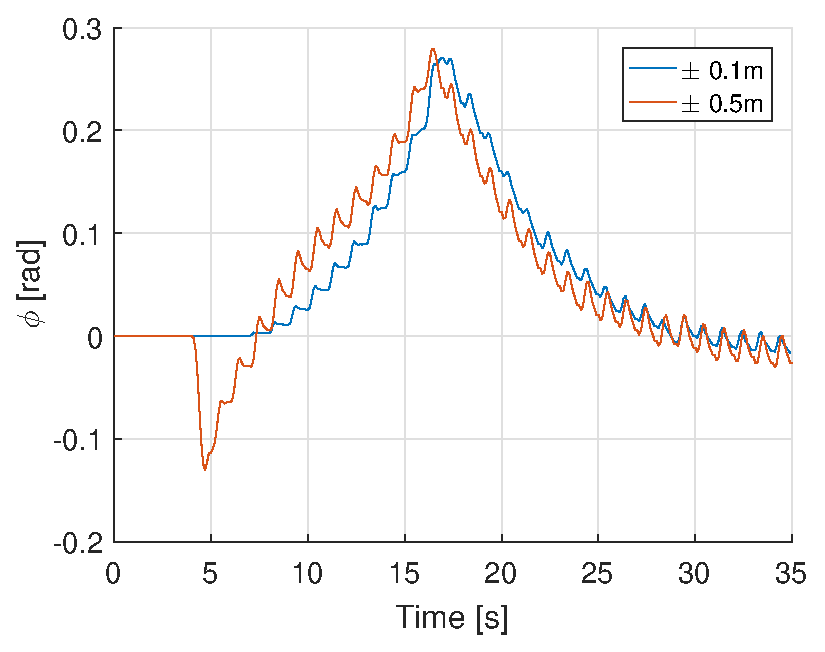
\includegraphics[width=0.8\textwidth, keepaspectratio=true]{../../results/opt/error/fig/attitude.eps}}
	\caption{The roll angle of the aircraft during a linear $45\degree$ turn with different acceptance rates for waypoints.}
	\label{fig:oscillating_attitude}
\end{figure}

In Figure \ref{fig:oscillating_attitude} the effect the acceptance range of waypoints has on the roll through a $45\degree$ linear turn is shown. When the acceptance range is $\pm 0.5$m, the magnitude of the oscillations is bigger than for an acceptance range of $\pm 0.1$m. A part from a spike in the wrong direction for the $\pm 0.5$m signal, the two roll angles follow approximately the same trajectory.


\section{Cost Function}

The cost function in this thesis consisted of eight states, where the position of the camera were the states included to solve the problem of finding an optimal path to track with a fixed camera. While this cost function do solve the problem, it does have some problems related to the tuning of it.

Early in testing, before the final tuning of the cost function had been decided, it was clear that the easiest way to solve the control problem was to control the course of the airplane using the rudder. This is an easy way to the problem since it does not rely on using the roll angle that inherently shifts the camera position. Since this thesis aimed to create an optimal path that could be used with a bank to turn controller, this behaviour had to be removed. This was done be heavily punishing usage of rudder, while there was almost no weight put on the usage of ailerons.

The tuning where the usage of rudder was punished did as intended: the MPC uses roll to follow the path instead of yaw. However, the light weighting of aileron input caused it to oscillate heavily, adding to the effect of the poor trajectory generation previously mentioned.

Another problem discovered during testing was how the MPC deals with long stretches of path. When the turns were positioned closely after one another it was no problem, but when optimizing the lawnmover path in section \ref{subsec:lawnmover} it became clear. The MPC chose to position the camera centre point on the ground path by keeping a constant roll angle and flying next to the path, and by keeping a constant deflection on the rudder it was able to maintain the course angle. Since the cost function only seek to minimize the control rates, this was a cheap solution.

One possible solution to this would be to include the position of the UAV in the cost function. These terms would have to weighted lower than the position of the camera since the camera position is the main focus, but it would cause flying next to the path a more expensive solution compared to flying just above the path. It could also have been avoided by included the rudder deflection as a term in the cost function.


\section{Comment on Control Signals}

\section{Different UAV Models Used}